\chapter{Related Work}
\label{chap:related-work}

This chapter provides an overview of the literature related to this dissertation.
\section{Probabilistic/Approximate design}
\label{sect:related-work-prob-approx}

While the shrinkage of device's feature size according to Moore's law~\cite{Moore1965}
has driven the prosperity of microelectronic industry,
the variability and uncertainty of devices at the atomic level
pose serious challenges on the continuation of the law.

New computational paradigms are proposed in response to the challenges in the post-Moore's era.
Among many other efforts,
along the direction of \textit{approximate design},
circuit architectures for
reconfigurable adders whose accuracy can be adjusted based on application scenarios~\cite{Kahng2012,Ye2013}
and energy-efficient adders with a moderate error rate~\cite{Kim2013} are proposed.
The automatic synthesis and analysis of approximate circuits have also been studied~\cite{Venkatesan2011ApproxDesign,Venkataramani2012,Miao2013,Miao2014,Li2014,Mrazek2016,Rehman2016}.
On the other hand, for \textit{probabilistic design},
Chakrapani et al.~\cite{Chakrapani2006ProbDesign} consider CMOS devices with probabilistic behavior,
establish the relation between energy consumption and probability of correct switching,
and exploit it to trade energy against correctness.

Despite the advancements made by prior endeavors, most of them focus on approximate design.
The analysis and synthesis of probabilistic design have gained relatively less attention.
Nevertheless, the study of probabilistic design is important in the following respects.
First, randomness is a valuable resource to trade for computation efficiency.
For example, there exist problems that can be solved efficiently by randomized algorithms
but not deterministic algorithms.
Second, there are applications, such as data mining, compressive sensing, etc.,
that may not be sensitive to minor random fluctuations.
Third, devices at their quantum foundation or systems in their biological nature are intrinsically probabilistic.
We aim at providing a formalism for the analysis and verification of probabilistic design.
Notice that in the design automation process,
verification is essential to the entire design flow.
For example, equivalence checking~\cite{Kuehlmann1997,Mishchenko2006}
should be applied to validate the correctness of synthesized circuits.
Hence, establishing a verification framework is a crucial step in automated synthesis of probabilistic design.

Probabilistic behavior of a design has also been studied along the research of circuit reliability analysis,
which focuses on analyzing the robustness of a circuit against permanent defects or transient faults.
The reliability of a circuit is characterized by the probability of the occurrence of an error at the primary outputs.
Therefore, the study of circuit reliability is very related to the evaluation of probabilistic design.

Classical approaches to reliability analysis apply fault injection and Monte Carlo simulation~\cite{Mohanram2003}.
Symbolic analysis methods exploiting mathematical tools,
such as Markov random fields~\cite{Bahar2003},
probability transfer matrices~\cite{Krishnaswamy2005},
Bayesian networks~\cite{Rejimon2005},
and algebraic decision diagrams~\cite{Miskov-Zivanov2006},
have also been investigated.
Choudhury and Mohanram~\cite{Choudhury2009} propose three accurate and scalable algorithms to address the scalability issue of symbolic methods.
However, prior methods for circuit reliability analysis are inadequate to probabilistic circuits
for the following two reasons.
First, most prior approaches assume single-gate failures.
This assumption makes prior methods inapplicable to probabilistic design,
where multiple probabilistic gates may be commonly present.
Second, most prior efforts consider only the average error rate of a design.
The necessity of analyzing the maximum error rate comes from the increasing demand of safety-centric systems,
e.g., utilized in health care or automotive industries~\cite{Lingasubramanian2007,Lingasubramanian2011}.
However, its computational scalability is much limited due to the underlying symbolic modeling via Bayesian network~\cite{Jensen1996}.
\begin{frame}
    \frametitle{Background}
    \begin{block}{Stochastic Boolean Satisfiability (SSAT)}
        $\Qf=Q_1 x_1,\ldots,Q_n x_n.\pf$
        \pause
        \begin{itemize}
            \item $Q_1 x_1,\ldots,Q_n x_n$: quantification structure, $Q_i \in \{\random{p},\exists\}$ (\emph{prefix})
                  \pause
            \item $\pf$: quantifier-free formula over $\{x_1,\ldots,x_n\}$ (\emph{matrix})
        \end{itemize}
    \end{block}
    \pause
    \begin{block}{Computational Rules for Satisfying Probability}
        Let $x$ be the outermost variable in the prefix:
        \pause
        \begin{enumerate}
            \item[a)] $\spb{\top}=1$,
                  \pause
            \item[b)] $\spb{\bot}=0$,
                  \pause
            \item[c)] $\spb{\Qf}=\max\{\spb{\ncf{\Qf}{x}},\spb{\pcf{\Qf}{x}}\}$, if $x$ is quantified by $\exists$,
                  \pause
            \item[d)] $\spb{\Qf}=(1-p)\spb{\ncf{\Qf}{x}}+p\spb{\pcf{\Qf}{x}}$, if $x$ is quantified by $\random{p}$.
        \end{enumerate}
    \end{block}
\end{frame}

\begin{frame}
    \frametitle{Background}
    \begin{block}{Example: Computation of Satisfying Probability}
        \abovedisplayskip=0pt
        \begin{align*}
             & \Qf=\random{0.5} x_1, \exists y_1, \random{0.5} x_2, \exists y_2. \pf \\
             & \pf=(x_1 \lor \lnot y_1)
            (\lnot x_1 \lor y_1)
            (\lnot x_1 \lor \lnot x_2 \lor y_2)
            (x_1 \lor \lnot y_2)
            (x_2 \lor \lnot y_2)
        \end{align*}
    \end{block}\pause
    \begin{figure}
        \centering
        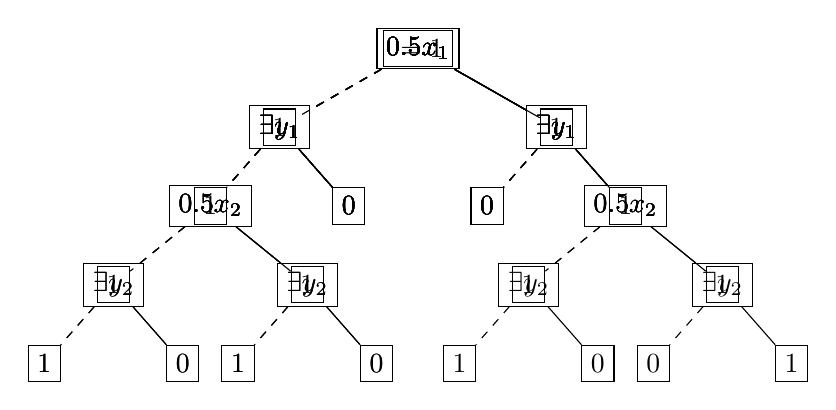
\begin{tikzpicture}[
                baseline,
                level distance=10mm,
                level 1/.style={sibling distance=10em},
                level 2/.style={sibling distance=5em},
                level 3/.style={sibling distance=7em},
                level 4/.style={sibling distance=5em},
                every node/.style={solid,draw},
                positive/.style={edge from parent/.style={solid,draw}},
                negative/.style={edge from parent/.style={dashed,draw}}]

            \action<2>{\node{$\random{0.5} x_1$};}
            \action<3>{\node{$\random{0.5} x_1$}
                child[negative]{node{$\exists y_1$}}
                child[positive]{node{$\exists y_1$}};}
            \action<4>{\node{$\random{0.5} x_1$}
                child[negative]{node{$\exists y_1$}
                        child[negative]{node{$\random{0.5} x_2$}}
                        child[positive]{node{$0$}}}
                child[positive]{node{$\exists y_1$}};}
            \action<5>{\node{$\random{0.5} x_1$}
                child[negative]{node{$\exists y_1$}
                        child[negative]{node{$\random{0.5} x_2$}}
                        child[positive]{node{$0$}}}
                child[positive]{node{$\exists y_1$}
                        child[negative]{node{$0$}}
                        child[positive]{node{$\random{0.5} x_2$}}};}
            \action<6>{\node{$\random{0.5} x_1$}
                child[negative]{node{$\exists y_1$}
                        child[negative]{node{$\random{0.5} x_2$}
                                child[negative]{node{$\exists y_2$}
                                        child[negative]{node{$1$}}
                                        child[positive]{node{$0$}}}
                                child[positive]{node{$\exists y_2$}
                                        child[negative]{node{$1$}}
                                        child[positive]{node{$0$}}}}
                        child[positive]{node{$0$}}}
                child[positive]{node{$\exists y_1$}
                        child[negative]{node{$0$}}
                        child[positive]{node{$\random{0.5} x_2$}}};}
            \action<7>{\node{$\random{0.5} x_1$}
                child[negative]{node{$\exists y_1$}
                        child[negative]{node{$\random{0.5} x_2$}
                                child[negative]{node{$\exists y_2$}
                                        child[negative]{node{$1$}}
                                        child[positive]{node{$0$}}}
                                child[positive]{node{$\exists y_2$}
                                        child[negative]{node{$1$}}
                                        child[positive]{node{$0$}}}}
                        child[positive]{node{$0$}}}
                child[positive]{node{$\exists y_1$}
                        child[negative]{node{$0$}}
                        child[positive]{node{$\random{0.5} x_2$}
                                child[negative]{node{$\exists y_2$}
                                        child[negative]{node{$1$}}
                                        child[positive]{node{$0$}}}
                                child[positive]{node{$\exists y_2$}
                                        child[negative]{node{$0$}}
                                        child[positive]{node{$1$}}}}};}
            \action<8>{\node{$\random{0.5} x_1$}
                child[negative]{node{$\exists y_1$}
                        child[negative]{node{$\random{0.5} x_2$}
                                child[negative]{node{$1$}}
                                child[positive]{node{$1$}}}
                        child[positive]{node{$0$}}}
                child[positive]{node{$\exists y_1$}
                        child[negative]{node{$0$}}
                        child[positive]{node{$\random{0.5} x_2$}
                                child[negative]{node{$1$}}
                                child[positive]{node{$1$}}}};}
            \action<9>{\node{$\random{0.5} x_1$}
                child[negative]{node{$\exists y_1$}
                        child[negative]{node{$1$}}
                        child[positive]{node{$0$}}}
                child[positive]{node{$\exists y_1$}
                        child[negative]{node{$0$}}
                        child[positive]{node{$1$}}};}
            \action<10>{\node{$\random{0.5} x_1$}
                child[negative]{node{$1$}}
                child[positive]{node{$1$}};}
            \action<11>{\node{$\spb{\Qf}=1$};}
        \end{tikzpicture}
    \end{figure}
\end{frame}

\begin{frame}
    \frametitle{Express Model-Counting Variants with SSAT}
    \begin{table}[t]
        \centering
        \begin{tabular}{c|c}
            Variant            & SSAT encoding                                                               \\
            \hline
            Unweighted         & $\random{0.5}x_1,\ldots,\random{0.5}x_n.\pf$                                \\
            Weighted           & $\random{p_1}x_1,\ldots,\random{p_n}x_n.\pf$                                \\
            Projected          & $\random{0.5}x_1,\ldots,\random{0.5}x_n,\exists y_1,\ldots,\exists y_m.\pf$ \\
            Maximum            & $\exists x_1,\ldots,\exists x_n,\random{0.5}y_1,\ldots,\random{0.5}y_m.\pf$ \\
            Projected weighted & $\random{p_1}x_1,\ldots,\random{p_n}x_n,\exists y_1,\ldots,\exists y_m.\pf$ \\
            Maximum weighted   & $\exists x_1,\ldots,\exists x_n,\random{p_1}y_1,\ldots,\random{p_m}y_m.\pf$ \\
        \end{tabular}
    \end{table}
\end{frame}

\begin{frame}
    \frametitle{Background}
    \begin{block}{Game-Theoretical Interpretation of SSAT}
        $\Qf=Q_1 x_1,\ldots,Q_n x_n.\pf$, $Q_i \in \{\random{p},\exists\}$
        \pause
        \begin{itemize}
            \item $\random{p}$: nondeterministic factors
                  \pause
            \item $\exists$: an agent who plays under uncertainty
                  \pause
            \item $\pf$: game matrix
                  \pause
            \item $\spb{\Qf}$: the maximum winning probability of the agent
                  \pause
            \item \alert{Skolem functions}: a winning/optimization strategy of the agent
        \end{itemize}
    \end{block}\pause
    \begin{block}{Example: Skolem Functions}
        \abovedisplayskip=0pt
        \belowdisplayskip=0pt
        \begin{align*}
             & \Qf=\random{0.5} x_1, \exists y_1, \random{0.5} x_2, \exists y_2. \pf \\
             & \pf=(x_1 \lor \lnot y_1)
            (\lnot x_1 \lor y_1)
            (\lnot x_1 \lor \lnot x_2 \lor y_2)
            (x_1 \lor \lnot y_2)
            (x_2 \lor \lnot y_2)
        \end{align*}
        \pause
        \begin{itemize}
            \item Variable $y_1$: $f_1(x_1)=x_1$; variable $y_2$: $f_2(x_1,x_2)=x_1 \land x_2$
        \end{itemize}
    \end{block}
\end{frame}
\section{Model counting}
\label{sect:related-work-model-counting}

Model-counting~\cite{SATHandbook-ModelCounting} algorithms can be classified into two categories:
exact counting and approximate counting.
The former adopts DPLL-based search with additional techniques,
such as component analysis and caching, to improve the counting efficiency\cite{Sang2004,Sang2005ModelCounting}.
The latter takes a different strategy,
aiming at providing lower and/or upper bounds with guarantee on confidence level.
Ideas from statistics~\cite{Chakraborty2016} have been adopted to increase the capacity limit of model counting.

There are many variants of model counting.
For example,
weighted model counting asks to aggregate the weight of every satisfying assignment.
It has been widely adopted in probabilistic inference~\cite{Sang2005BayesianInference,Chavira2008}.
\textit{Projected model counting}~\cite{Aziz2015} computes the numbers of satisfying assignments
projected on a subset of original variables.
\textit{Maximum model counting}~\cite{Fremont2017} finds an assignment to a subset of variables in a formula
such that the number of satisfying assignments of the residual formula cofactored with the assignment is maximized.

The above variants of model counting can be expressed via SSAT,
because the randomized quantifiers of SSAT essentially aggregate the results from different branches with weights.
\Cref{tbl:related-work-model-counting} shows the variants of model-counting problems and their respective SSAT encodings.
Note that projected weighted model counting and maximum weighted model counting are equivalent to
random-exist quantified SSAT and exist-random quantified SSAT, respectively.

\begin{table}[t]
    \centering
    \caption{Model-counting variants and their corresponding SSAT formulas}
    \label{tbl:related-work-model-counting}
    \begin{tabular}{c|c}
        Model-counting variant & SSAT encoding                                                                                              \\
        \hline
        Unweighted             & $\random{0.5}x_1,\ldots,\random{0.5}x_n.\pf(x_1,\ldots,x_n)$                                               \\
        Weighted               & $\random{p_1}x_1,\ldots,\random{p_n}x_n.\pf(x_1,\ldots,x_n)$                                               \\
        Projected              & $\random{0.5}x_1,\ldots,\random{0.5}x_n,\exists y_1,\ldots,\exists y_m.\pf(x_1,\ldots,x_n,y_1,\ldots,y_m)$ \\
        Maximum                & $\exists x_1,\ldots,\exists x_n,\random{0.5}y_1,\ldots,\random{0.5}y_m.\pf(x_1,\ldots,x_n,y_1,\ldots,y_m)$ \\
        Projected weighted     & $\random{p_1}x_1,\ldots,\random{p_n}x_n,\exists y_1,\ldots,\exists y_m.\pf(x_1,\ldots,x_n,y_1,\ldots,y_m)$ \\
        Maximum weighted       & $\exists x_1,\ldots,\exists x_n,\random{p_1}y_1,\ldots,\random{p_m}y_m.\pf(x_1,\ldots,x_n,y_1,\ldots,y_m)$ \\
    \end{tabular}
\end{table}

The latest developments of model counting can be found in the report~\cite{MC-COMP2020} of the 2020 Model Counting Competition.

\iffalse
    with pruning heuristics and subproblem memorization
    For example, \maxplan~\cite{Majercik1998} improves the DPLL-based search by considering pure literal, unit propagation, and subproblem memorization;
    \zander~\cite{Majercik2003} incorporates several threshold pruning heuristics to reduce the search space;
    \dcssat~\cite{Majercik2005} divides the SSAT formulas into many subproblems and conquer them separately.
\fi

\iffalse
    \section{Introduction of the AAAI '21 paper}
    Satisfiability (SAT) solvers~\cite{SATHandbook} have been successfully applied to numerous research fields including artificial intelligence~\cite{Nilsson2014,Russell2020}, electronic design automation~\cite{Marques2000,Wang2009}, software verification~\cite{Jhala2009, Berard2013}, etc.
    The tremendous benefits have encouraged the development of more advanced decision procedures for satisfiability with respect to more complex logics beyond pure propositional.
    For example, solvers of the satisfiability modulo theories (SMT)~\cite{Moura2011,HBMC-SMT} accommodate first order logic fragments; quantified Boolean formula (QBF)~\cite{Narizzano2006,SATHandbook-QBF} allows both existential and universal quantifiers; stochastic Boolean satisfiability (SSAT)~\cite{Littman2001,SATHandbook-SSAT} models uncertainty with random quantification; and dependency QBF (DQBF)~\cite{Balabanov2014,Scholl2018} equips Henkin quantifiers to describe multi-player games with partial information.
    Due to their simplicity and generality, various satisfiability formulations are under active investigation.

    Among the quantified decision procedures, QBF and SSAT are closely related.
    While SSAT extends QBF to allow random quantifiers to model uncertainty, they are both PSPACE-complete~\cite{Stockmeyer1973}.
    A number of SSAT solvers have been developed and applied in probabilistic planning, formal verification of probabilistic design, partially observable Markov decision process (POMDP), and analysis of software security.
    For example, solver \texttt{MAXPLAN}~\cite{Majercik1998} encodes a conformant planning problem as an exist-random quantified SSAT formula; solver \texttt{ZANDER}~\cite{Majercik2003} deals with partially observable probabilistic planning by formulating the problem as a general SSAT formula; solver \texttt{DC-SSAT}~\cite{Majercik2005} relies on a divide-and-conquer approach to speedup the solving of a general SSAT formula.
    Solvers \texttt{ressat} and \texttt{erssat}~\cite{LeeIJCAI17RESSAT,LeeIJCAI18ERSSAT} are developed for random-exist and exist-random quantified SSAT formulas respectively, and applied to the formal verification of probabilistic design~\cite{LeeTC18ProbDesign}.
    POMDP has also been studied under the formalism of SSAT~\cite{Majercik2004,Salmon2020}.
    Recently, bi-directional polynomial-time reductions between SSAT and POMDP are established~\cite{Salmon2020}.
    The quantitative information flow analysis for software security is also investigated as an exist-random quantified SSAT formula~\cite{Fremont2017}.

    In view of the close relation between QBF and SSAT, we raise the question what would be the formalism that extends DQBF to the stochastic domain.
    We formalize the \emph{dependency SSAT} (DSSAT) as the answer to the question.
    We prove that DSSAT has the same NEXPTIME-complete complexity as DQBF~\cite{Peterson2001}, and therefore it can succinctly encode decision problems with uncertainty in the NEXPTIME complexity class.

    To highlight the benefits of DSSAT over DQBF, we note that DSSAT intrinsically represents an optimization problem (the answer is the maximum satisfying probability) while DQBF is a decision problem (the answer is either true or false).
    The optimization nature of DSSAT potentially allows broader applications of the formalism.
    Moreover, DSSAT is often preferable to DQBF in expressing problems involving uncertainty and probabilities.
    As case studies, we investigate its applicability in probabilistic system design/verification and artificial intelligence.

    In system design of the post Moore's law era, the practice of \textit{very large scale integration} (VLSI) circuit design experiences a paradigm shift in design principles to overcome the obstacle of physical scaling of computation capacity.
    Probabilistic design~\cite{Chakrapani2006ProbDesign} and approximate design~\cite{Venkatesan2011ApproxDesign} are two such examples of emerging design methodologies.
    The former does not require logic gates to be error-free, but rather allowing them to function with probabilistic errors.
    The latter does not require the implementation circuit to behave exactly the same as the specification, but rather allowing their deviation to some extent.
    These relaxations to design requirements provide freedom for circuit simplification and optimization.
    We show that DSSAT can be a useful tool for the analysis of probabilistic design and approximate design.

    The theory and applications of Markov decision process and its variants are among the most important topics in the study of artificial intelligence.
    For example, the decision problem involving multiple agents with uncertainty and partial information is often considered as a decentralized POMDP (Dec-POMDP)~\cite{Oliehoek2016}.
    The independent actions and observations of the individual agents make POMDP for single-agent systems not applicable and require the more complex Dec-POMDP.
    Essentially the complexity is lifted from the PSPACE-complete policy evaluation of finite-horizon POMDP to the NEXPTIME-complete Dec-POMDP.
    We show that Dec-POMDP is polynomial time reducible to DSSAT.

    \section{Introduction of the IJCAI '18 paper}
    \textit{Stochastic Boolean satisfiability} (SSAT) was first formulated by Papadimitriou and interpreted as \emph{games against nature}~\cite{Papadimitriou1985}.
    In an SSAT formula, a Boolean variable can be \textit{randomly quantified with probability $p$} by a \textit{randomized quantifier}, which specifies that the variable evaluates to \textsc{true} with probability $p$.
    With randomized quantifiers, SSAT serves as a natural formalism for an abundance of computational problems endowed with randomness, such as propositional probabilistic planning, trust management, and Bayesian network inference~\cite{Littman2001,SATHandbook-SSAT,Hnich2011}.
    The verification problem of VLSI circuits with probabilistic errors has also been investigated under the framework of SSAT recently~\cite{LeeTC18ProbDesign}.
    From the perspective of computational complexity, SSAT lies in the complexity class PSPACE-complete, the same as quantified Boolean formula (QBF).
    Therefore, advancing the scalability of SSAT solving not only benefits practical applications, but also has profound theoretical values.

    In this paper, we focus on the exist-random quantified SSAT formulas of the form $\Phi=\exists X \random{} Y.\phi$, which is known as \emph{E-MAJSAT}~\cite{Littman1998}.
    %E-MAJSAT is in the $\mathrm{NP}^\mathrm{PP}$-complete complexity class.
    Computational problems, such as computing a \textit{maximum a posteriori}
    (MAP) hypothesis or a \textit{maximum expected utility} (MEU) solution~\cite{Dechter1998} in belief networks, and searching an optimal plan for probabilistic conformant planning domains~\cite{Littman1998}, can be formulated with E-MAJSAT.

    Among previous endeavors, several techniques have been investigated to solve SSAT.
    Prior work \texttt{MAXPLAN}~\cite{Majercik1998} utilizes Davis-Putnam-Logemann-Loveland (DPLL) search~\cite{Davis1962} and improves its efficiency by considering pure variables, unit propagation, and subproblem memorization.
    \texttt{DCSSAT}~\cite{Majercik2005} enhances \texttt{MAXPLAN} by applying the divide-and-conquer strategy to break SSAT formulas into many subproblems and solve them separately.
    %The solution of the original formula is built based on the solutions to solved subproblems.
    The technique of \textit{knowledge compilation} has also been exploited to solve E-MAJSAT.
    \texttt{ComPlan}~\cite{Huang2006} compiles the problems into \textit{deterministic, decomposable negation normal form} (d-DNNF)~\cite{Darwiche2001,Darwiche2002dDNNF}, and performs a branch-and-bound search.
    It is further improved by an enhanced bound computation method~\cite{Pipatsrisawat2009}.
    Recent work~\cite{Fremont2017} proposed a \textit{maximum model counting} algorithm for solving a special case of E-MAJSAT with all probabilities of randomized quantifiers equal to $0.5$.
    Recently, modern SAT techniques have been utilized to solve random-exist quantified SSAT formulas~\cite{LeeIJCAI17RESSAT}, which inspires us to examine the possibility of applying QBF solving techniques in the SSAT domain.

    In this paper, we exploit the \textit{clause selection} technique, which has been introduced in QBF solving recently \cite{Janota2015,Rabe2015}, and
    propose a \textit{clause containment learning} method for E-MAJSAT solving.
    To the best of our knowledge, this paper is the first attempt to adopt approaches developed for QBF to solve SSAT.
    In addition to the learning technique, weighted model counting, which has been widely adopted in probabilistic inference~\cite{Sang2005BayesianInference,Chavira2008}, is utilized in the proposed algorithm to compute probabilities.
    The scalability of model counting has been improved under the paradigm of approximate counting~\cite{Chakraborty2016} over its conventional exact counterpart~\cite{Sang2004,Sang2005ModelCounting}.

    We evaluate the proposed algorithm with a wide range of benchmarks including random formulas,
    planning problems, and probabilistic circuit verification.
    Experiments show that our method achieves significant performance gains and memory savings compared to the state-of-the-art SSAT solvers.

    \section{Introduction of the IJCAI '17 paper}
    First formulated by Papadimitriou~\cite{Papadimitriou1985}, \textit{stochastic Boolean satisfiability} (SSAT) was described as a game against nature.
    Probabilistic factors are introduced into the world of Boolean logic through the creation of the \textit{randomized quantifier}.
    A Boolean variable randomly quantified with probability $p$ has a probability $p$ of evaluating to \textsc{true}.
    Exploiting randomized quantifiers, SSAT is capable of modeling a variety of computational problems inherent with uncertainty~\cite{Hnich2011}, such as propositional probabilistic planning, belief network inference, and trust management~\cite{SATHandbook-SSAT}.
    Recently, it has also been applied to the formal verification of probabilistic circuits~\cite{LeeTC18ProbDesign}.
    From computational complexity point of view, SSAT lies in the PSPACE-complete complexity class, same as solving quantified Boolean formulas (QBF).
    Therefore, developing good algorithms for SSAT not only brings practical benefits for real-world applications, but also is of theoretical interest.

    Among the prior efforts made to approach SSAT, most of them are based on Davis-Putnam-Logemann-Loveland (DPLL) search~\cite{Davis1962}.
    \texttt{MAXPLAN}~\cite{Majercik1998} improves DPLL-based search by considering pure literal, unit propagation, and subproblem memorization.
    \texttt{ZANDER}~\cite{Majercik2003} incorporates several threshold pruning heuristics to reduce the search space.
    \texttt{DC-SSAT}~\cite{Majercik2005} divides the SSAT formulas into many subproblems and conquer them separately.
    The solution of the original formula is then constructed on top of the solutions of subproblems.
    \textit{Approximate SSAT} solving, which derives upper or lower bounds of satisfying probability of an SSAT formula instead of solving it exactly, was investigated~\cite{Majercik2007}.
    Resolution for SSAT has also been addressed~\cite{Teige2010}.

    On the other hand, model counting algorithms are under active development in recent years.
    In addition to \textit{exact model counting}~\cite{Sang2004,Sang2005ModelCounting},
    \textit{approximate model counting}~\cite{Gomes2006,Gomes2007,Chakraborty2016} has been addressed to improve scalability by relaxing exactness.
    In this work, exact or approximate model counting is exploited as an ingredient for SSAT solving.

    In contrast to the prior DPLL-based SSAT algorithms with pruning heuristics and subproblem memorization, our goal is to take advantage of modern SAT solvers~\cite{Een2003Solver,Een2003Incremental} and model counters as a blackbox engine for solving SSAT.
    To the best of our knowledge, this work is the first attempt to directly use a SAT solver as a plug-in engine for SSAT solving.
    In this paper, we focus on the random-exist quantified SSAT formula of the form $\Phi=\random{} X \exists Y.\phi$, which is the counterpart of the forall-exist quantified QBF formula.
    The random-exist quantified SSAT has applications in belief network inference~\cite{Cooper1990,Bacchus2003}, probabilistic planning, and probabilistic circuit verification~\cite{LeeTC18ProbDesign}.
    In addition to SAT solving, we incorporate weighted model counting, which has been widely used in probabilistic inference~\cite{Sang2005BayesianInference,Chavira2008}, in the proposed algorithm to tackle randomized quantifiers.
    The proposed algorithm uses the SAT solver and model counter in a \textit{stand-alone} manner, leaving the internal structures of these solvers intact.
    Due to the stand-alone usage of these solvers, the proposed algorithm may directly benefit from the advancement of the solvers without any modification.
    Moreover, unlike previous DPLL-based methods, the proposed algorithm can be easily modified to solve \textit{approximate SSAT} by deriving upper and lower bounds of satisfying probability.
    Furthermore, the proposed method can be applied to solve \textit{projected model counting}~\cite{Aziz2015}, which computes the numbers of satisfying assignments projected on a subset of original variables, because it is subsumed by random-exist quantified SSAT.

    To evaluate the proposed algorithm, a prototype program was implemented and experimented with random $k$-CNF formulas, \textit{strategic companies}~\cite{Cadoli1997} formulas arising from the artificial intelligence (AI) domain, and benchmarks from analysis of very-large-scale integration (VLSI) circuits.
    Our method outperforms the state-of-the-art algorithm on random $k$-CNF and strategic companies formulas in both runtime and memory consumption, and is capable of solving approximate SSAT on circuit benchmarks while the state-of-the-art method fails to compute the exact satisfying probability.

    \section{Introduction of the TC '18 paper}
    The shrinkage of device's feature size according to Moore's law~\cite{Moore1965} has driven the prosperity of microelectronic industry.
    The more transistors we cram into an IC, the more complex system we can realize.
    The main reason behind all these benefits arises from device scaling;
    therefore, it is a significant research issue to keep this desirable trend.

    The continuation of Moore's law has encountered some difficulty.
    The variability and uncertainty of manufacturing at the atomic level make devices under miniaturization sensitive to process variation and environmental fluctuation.
    Moreover, lowering supply voltages decreases noise margin and makes an integrated circuit (IC) susceptible to noise.
    As a result, the manufactured ICs may exhibit uncertain probabilistic behavior,
    which imposes serious challenges to the design of reliable systems.

    Conventionally, uncertain system behavior is undesirable and would be mitigated by employing techniques such as error detection~\cite{Constantinescu2003} and error correction~\cite{Mitra2006}.
    However, there has been a paradigm shift to accept inevitable imperfection.
    For example, the 2007 report of the International Technology Roadmap for Semiconductors (ITRS)
    acknowledges
    ``\textit{Relaxing the requirement of $100\%$ correctness for devices and interconnects may dramatically reduce the costs of manufacturing, verification, and test.
        Such a paradigm shift is likely forced in any case by technology scaling, which leads to more transient and permanent failures of signals, logic values, devices, and interconnects.}''

    Recent research efforts have been made along this direction based
    on the notions of \textit{approximate design} and \textit{probabilistic design}.
    In both notions, a system's behavior may deviate from its expected specification;
    however, this deviation is deterministic in the former case but probabilistic in the latter case.
    Among many other efforts, prior work~\cite{Chakrapani2006ProbDesign} considered CMOS devices with probabilistic behavior, established the relation between energy consumption and probability of correct switching, and exploited it to trade energy against correctness.
    Reconfigurable adders, whose accuracy can be adjusted depending on application scenarios, were proposed~\cite{Kahng2012,Ye2013}.
    An energy efficient approximate adder with a moderate error rate was proposed~\cite{Kim2013}.
    The synthesis of approximate circuits have been studied~\cite{Venkatesan2011ApproxDesign,Venkataramani2012,Miao2013,Miao2014};
    the analysis of approximate arithmetic circuits have been explored~\cite{Li2014,Mrazek2016,Rehman2016}.
    (In the sequel, the term ``design'' is used as a general term that refers to a single design instance, a set of design instances, or design process;
    the term ``synthesis" is referred to as the design automation process transforming a system under design from high-level system specification to low-level circuit implementation.)

    Despite the advancements made by prior endeavors, most of them focused on approximate design.
    The analysis and synthesis of probabilistic design gained relatively less attention.
    Nevertheless the study of probabilistic design can be important in the following respects.
    First, randomness can be a valuable resource to trade for computation efficiency.
    For example, there exist problems that can be solved efficiently by randomized algorithms, but not deterministic algorithms.
    Second, there are applications, such as data mining, compressive sensing, etc., that may not be
    sensitive to minor random fluctuations.
    Third, devices at their quantum foundation or systems in their biological nature are intrinsically probabilistic.
    This paper aims to provide a formalism for the analysis and verification of probabilistic design.
    Notice that in the design automation process, verification is essential to the entire design flow.
    For example, equivalence checking~\cite{Kuehlmann1997,Mishchenko2006} should be applied to validate the correctness of synthesized circuits.
    Hence, establishing a verification framework is a crucial step in automated synthesis of probabilistic design.

    Probabilistic behavior of a design has also been studied along the research of circuit reliability analysis, which focuses on analyzing the robustness of a circuit against permanent defects or transient faults.
    The reliability of a circuit is characterized by the probability of the occurrence of an error at the primary outputs.
    Therefore, the study of circuit reliability is very related to the evaluation of probabilistic design.
    (In the sequel, the terms ``analysis'' and ``evaluation'' are used interchangeably as general terms referring to the process of determining qualitative or quantitative properties of a design.
    We will formulate the problem of \textit{probabilistic property evaluation}, and refer to the term ``evaluation" as computing the satisfying probability of certain properties of a probabilistic design.)
    Classical approaches to reliability analysis apply fault injection and Monte Carlo simulation~\cite{Mohanram2003}.
    Symbolic analysis methods exploiting mathematical tools, such as Markov random fields~\cite{Bahar2003}, probability transfer matrices~\cite{Krishnaswamy2005}, Bayesian networks~\cite{Rejimon2005}, and algebraic decision diagrams~\cite{Miskov-Zivanov2006}, have also been investigated.
    Three accurate and scalable algorithms were proposed~\cite{Choudhury2009} to address the scalability issue of symbolic methods.
    However, prior methods for circuit reliability analysis are inadequate to probabilistic circuits for the following two reasons.
    First, most prior approaches assume single-gate failures.
    This assumption makes prior methods inapplicable to probabilistic design, where multiple probabilistic gates may be commonly present.
    Second, most prior efforts consider only the average error rate of a design.
    The necessity of analyzing the maximum error rate comes from the increasing demand of safety-centric systems, e.g., utilized in health care or automotive industries~\cite{Lingasubramanian2007,Lingasubramanian2011}.
    However, its computational scalability was much limited due to the underlying symbolic modeling via Bayesian network~\cite{Jensen1996}.
    As will be shown in the experiments, our proposed method outperforms the previous works~\cite{Lingasubramanian2007,Lingasubramanian2011} by orders of magnitude in terms of both runtime and memory usage, and thus provides a scalable framework to analyze more expressive properties of probabilistic design, including both average and maximum error rates.

    In this paper, we formalize the problem of probabilistic property evaluation and provide different computation solutions.
    In the proposed probabilistic property evaluation framework, no restriction is imposed on the number of gates with probabilistic errors.
    We exploit stochastic Boolean satisfiability (SSAT) for both average-case and worst-case analyses.
    For average-case property evaluation, we additionally present solutions based on model counting, and probabilistic model checking.
    Moreover, a novel SSAT solver based on binary decision diagram (BDD) is developed.
    We perform experimental evaluation to compare different solutions.
    Among the proposed techniques, the BDD-based SSAT solver achieves the best scalability in our experiments.
    On the other hand, our formula-rewriting technique is crucial for approximate weighted model counting to be applicable, and uniquely resolves some cases, which cannot be solved efficiently by other alternative methods.
\fi